% Chapter Template

\chapter{Data Sources} % Main chapter title

\label{Chapter3} % Change X to a consecutive number; for referencing this chapter elsewhere, use \ref{ChapterX}

%----------------------------------------------------------------------------------------
%	SECTION 1
%----------------------------------------------------------------------------------------

\section{Data on Government support}

This thesis uses data from european state aid transparency database \parencite{eu_com_state_2023}. 
The data base contains information about individual award data like beneficiary name, amount, Date of Granting, and the purpose of the state aid \parencite{eu_com_state_2023}. 

The legal base for the transparency requirement aid payments is Temporary Framework for State aid, however payments under 100.000 EUR (10.000 EUR for agricultural firm) are exempted from the transparency requirement, insofar the data base is not comprehensive. Nevertheless, as of spring 2023 for Germany 135.478 cases of aid related to the COVID-19 pandemic were disclosed under the objective “Remedy for a serious disturbance in the economy”. Unfortunately, the disclosed titles of the aid measures and case numbers doesn't allow for reconciliation to the official names of the aid programs due to amendments and overlaps. In addition, in case of bigger companies the aid was usually calculated on a group level but awarded and paid in full to just one company of the group. 

Another thing to be mentioned is that most direct grants were granted and paid on a provisional basis and are still subject to a final determination of the granted amount. For the research this doesn't pose an issue, since the effects of payments will be observable regardless whether the amount of aid got adjusted in later period. 





%----------------------------------------------------------------------------------------
%	SECTION 2
%----------------------------------------------------------------------------------------

\section{Company level financial information}

In Germany corporations are legally required to disclose their annual financial statements in the Federal Gazette. Although the discloser of financial information is legally required for corporations, in there are various exemption for example for companies that are consolidated into other companies' balance sheets, and also non-compliant companies.
The requirement on the disclosed financial information is depending on the size of the company. Bigger companies above certain thresholds additionally need disclose their profit and loss statements and management report additionally. However, all companies that are subject of regulation must disclose at least their balance sheet. 
To not exclude SMEs systematically, due to missing profit and loss statements, the data collection process is limited to balance sheet information. 

The main constraint in processing the financial information from the Federal Gazette is the vastly unstandardized formatting of balance sheets causing limited readability in the data parsing step. By scraping and parsing the financial information for beneficiaries of pandemic government support balance sheets of 23.505 companies for at least one year in the period 2018 - 2022 was obtained. Figure \ref{fig:FirmSizes} shows that SMEs are represented in dataset and that the distribution between 2020 and 2021 is comparable.

It is necessary to mention, that in cases of two companies of the same name the matching is prone to mismatches and information for registry numbers of firms for validation was not consistently available in the database on state aid.

\begin{figure}
    \centering
    \makebox[\textwidth][c]{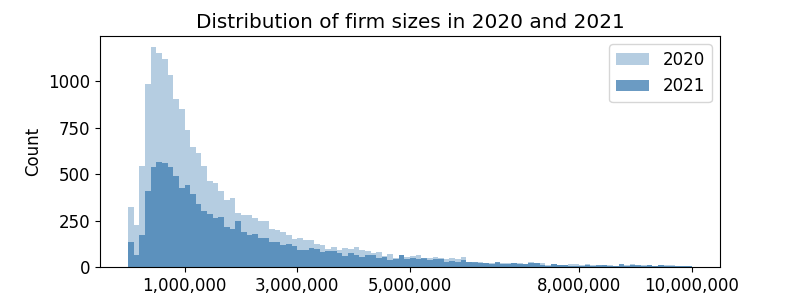
\includegraphics[width=1\columnwidth]{Figures/FirmSizes}}%
    
    \decoRule
    \caption[Firm size distribution in dataset]{Histogram shows the distribution of total asset as a proxy for the size of the firms in the dataset. The X axis is cut off at 10 mio. Euros.}
    \label{fig:FirmSizes}
\end{figure}


%----------------------------------------------------------------------------------------
%	SECTION 3
%----------------------------------------------------------------------------------------

\section{Insolvency information}

To further understand how effective the aid measures were in preventing insolvencies, data on insolvencies in Germany was obtained from the insolvencies notification platform and matched with the beneficiaries of government support on the state aid transparency database. 
The data from the insolvencies notification platform data was used for the matching ranges from 2020 to March 2023. Like with the matching of financial information with the beneficiaries, matching was also prone to mismatches in case of two companies of the same name.

